

\tikzset{every picture/.style={line width=0.75pt}} %set default line width to 0.75pt        

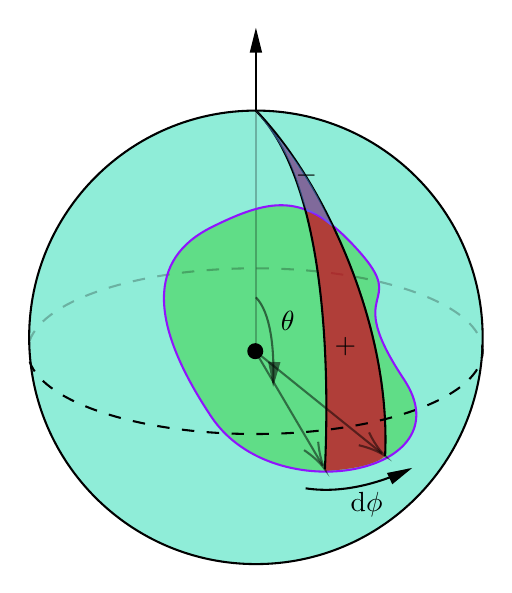
\begin{tikzpicture}[x=0.75pt,y=0.75pt,yscale=-1,xscale=1]
%uncomment if require: \path (0,300); %set diagram left start at 0, and has height of 300

%Shape: Polygon Curved [id:ds889444292321216] 
\draw  [draw opacity=0][fill={rgb, 255:red, 126; green, 211; blue, 33 }  ,fill opacity=1 ] (349.96,114.76) .. controls (380.36,99.55) and (396.23,98.36) .. (420.97,126.12) .. controls (445.71,153.88) and (412.3,142.26) .. (442.71,187.88) .. controls (473.11,233.49) and (380.36,251.6) .. (349.96,205.99) .. controls (319.55,160.37) and (319.55,129.96) .. (349.96,114.76) -- cycle ;
%Shape: Circle [id:dp8581661227878492] 
\draw  [fill={rgb, 255:red, 80; green, 227; blue, 194 }  ,fill opacity=0.64 ] (262.21,167.75) .. controls (262.21,107.41) and (311.12,58.5) .. (371.46,58.5) .. controls (431.79,58.5) and (480.71,107.41) .. (480.71,167.75) .. controls (480.71,228.09) and (431.79,277) .. (371.46,277) .. controls (311.12,277) and (262.21,228.09) .. (262.21,167.75) -- cycle ;
%Shape: Arc [id:dp6972719223448967] 
\draw  [draw opacity=0][dash pattern={on 4.5pt off 4.5pt}] (480.45,177.11) .. controls (480.62,176.23) and (480.7,175.33) .. (480.7,174.42) .. controls (480.7,152.38) and (431.66,134.5) .. (371.16,134.49) .. controls (315.32,134.48) and (269.23,149.69) .. (262.46,169.37) -- (371.15,174.41) -- cycle ; \draw  [color={rgb, 255:red, 0; green, 0; blue, 0 }  ,draw opacity=0.25 ][dash pattern={on 4.5pt off 4.5pt}] (480.45,177.11) .. controls (480.62,176.23) and (480.7,175.33) .. (480.7,174.42) .. controls (480.7,152.38) and (431.66,134.5) .. (371.16,134.49) .. controls (315.32,134.48) and (269.23,149.69) .. (262.46,169.37) ;
%Shape: Polygon Curved [id:ds04081945273310117] 
\draw  [draw opacity=0][fill={rgb, 255:red, 208; green, 2; blue, 27 }  ,fill opacity=0.72 ] (371.46,58.5) .. controls (424.46,120.75) and (436.46,186.4) .. (433.71,224.88) .. controls (429.36,228.8) and (420.56,231) .. (404.76,232.2) .. controls (404.96,202) and (410.06,98.35) .. (371.46,58.5) -- cycle ;
%Straight Lines [id:da7663338765803891] 
\draw    (371.46,20.61) -- (371.46,58.5) ;
\draw [shift={(371.46,18.61)}, rotate = 90] [fill={rgb, 255:red, 0; green, 0; blue, 0 }  ][line width=0.08]  [draw opacity=0] (12,-3) -- (0,0) -- (12,3) -- cycle    ;
%Straight Lines [id:da17557786530162556] 
\draw [color={rgb, 255:red, 0; green, 0; blue, 0 }  ,draw opacity=0.25 ]   (371.46,58.5) -- (371.46,172.53) ;
%Shape: Arc [id:dp2902499002256753] 
\draw  [draw opacity=0][dash pattern={on 4.5pt off 4.5pt}] (480.45,171.7) .. controls (480.62,172.58) and (480.7,173.48) .. (480.7,174.39) .. controls (480.7,196.43) and (431.66,214.31) .. (371.16,214.33) .. controls (315.32,214.34) and (269.23,199.12) .. (262.46,179.44) -- (371.15,174.41) -- cycle ; \draw  [dash pattern={on 4.5pt off 4.5pt}] (480.45,171.7) .. controls (480.62,172.58) and (480.7,173.48) .. (480.7,174.39) .. controls (480.7,196.43) and (431.66,214.31) .. (371.16,214.33) .. controls (315.32,214.34) and (269.23,199.12) .. (262.46,179.44) ;
%Shape: Polygon Curved [id:ds25655974777088986] 
\draw  [color={rgb, 255:red, 144; green, 19; blue, 254 }  ,draw opacity=1 ] (349.96,114.76) .. controls (380.36,99.55) and (396.23,98.36) .. (420.97,126.12) .. controls (445.71,153.88) and (412.3,142.26) .. (442.71,187.88) .. controls (473.11,233.49) and (380.36,251.6) .. (349.96,205.99) .. controls (319.55,160.37) and (319.55,129.96) .. (349.96,114.76) -- cycle ;
%Straight Lines [id:da7340832576388971] 
\draw [color={rgb, 255:red, 0; green, 0; blue, 0 }  ,draw opacity=0.5 ][line width=0.75]    (432.15,223.62) -- (371.15,174.41) ;
\draw [shift={(433.71,224.88)}, rotate = 218.9] [color={rgb, 255:red, 0; green, 0; blue, 0 }  ,draw opacity=0.5 ][line width=0.75]    (13.12,-3.95) .. controls (8.34,-1.68) and (3.97,-0.36) .. (0,0) .. controls (3.97,0.36) and (8.34,1.68) .. (13.12,3.95)   ;
%Straight Lines [id:da9654246631096741] 
\draw    (262,160.95) ;
%Straight Lines [id:da4149840059520884] 
\draw    (371.15,174.41) ;
\draw [shift={(371.15,174.41)}, rotate = 0] [color={rgb, 255:red, 0; green, 0; blue, 0 }  ][fill={rgb, 255:red, 0; green, 0; blue, 0 }  ][line width=0.75]      (0, 0) circle [x radius= 3.35, y radius= 3.35]   ;
%Straight Lines [id:da01982672141711772] 
\draw [color={rgb, 255:red, 0; green, 0; blue, 0 }  ,draw opacity=0.5 ][line width=0.75]    (403.69,229.66) -- (371.15,174.41) ;
\draw [shift={(404.71,231.38)}, rotate = 239.51] [color={rgb, 255:red, 0; green, 0; blue, 0 }  ,draw opacity=0.5 ][line width=0.75]    (13.12,-3.95) .. controls (8.34,-1.68) and (3.97,-0.36) .. (0,0) .. controls (3.97,0.36) and (8.34,1.68) .. (13.12,3.95)   ;
%Curve Lines [id:da8815428682205915] 
\draw    (395.4,240.49) .. controls (415.04,243.5) and (433.96,236.55) .. (445.04,231.46) ;
\draw [shift={(446.73,230.68)}, rotate = 514.62] [fill={rgb, 255:red, 0; green, 0; blue, 0 }  ][line width=0.08]  [draw opacity=0] (12,-3) -- (0,0) -- (12,3) -- cycle    ;
%Curve Lines [id:da13646790679271525] 
\draw    (371.46,58.5) .. controls (401.71,89.49) and (407.71,165.49) .. (404.71,231.38) ;
%Curve Lines [id:da6797173532010126] 
\draw    (371.46,58.5) .. controls (401.71,89.49) and (436.71,158.99) .. (433.71,224.88) ;
%Curve Lines [id:da005763715874352204] 
\draw [color={rgb, 255:red, 0; green, 0; blue, 0 }  ,draw opacity=0.54 ]   (371.46,148.49) .. controls (378.7,155.91) and (380.36,173.67) .. (379.82,189.61) ;
\draw [shift={(379.75,191.59)}, rotate = 272.61] [fill={rgb, 255:red, 0; green, 0; blue, 0 }  ,fill opacity=0.54 ][line width=0.08]  [draw opacity=0] (12,-3) -- (0,0) -- (12,3) -- cycle    ;
%Shape: Polygon Curved [id:ds20323205521229104] 
\draw  [draw opacity=0][fill={rgb, 255:red, 74; green, 144; blue, 226 }  ,fill opacity=0.52 ] (371.46,58.5) .. controls (391.29,83.21) and (390.49,93.61) .. (396.09,107.21) .. controls (403.69,108.01) and (404.09,112.01) .. (408.49,114.41) .. controls (400.49,99.21) and (398.89,90.81) .. (371.46,58.5) -- cycle ;

% Text Node
\draw (382,153.69) node [anchor=north west][inner sep=0.75pt]    {$\theta $};
% Text Node
\draw (424.79,240.69) node [anchor=north] [inner sep=0.75pt]    {$\mathrm{d} \phi $};
% Text Node
\draw (407.88,166.09) node [anchor=north west][inner sep=0.75pt]    {$+$};
% Text Node
\draw (389.08,84.09) node [anchor=north west][inner sep=0.75pt]    {$-$};


\end{tikzpicture}
